\documentclass{article}
\usepackage{geometry}
\usepackage{amsmath}
\usepackage{amsfonts}
\usepackage{amssymb}
\usepackage{amsthm}
\usepackage{parskip}
\usepackage{multicol}
\usepackage{xcolor}
\usepackage{fancyhdr}
\usepackage{physics}
\usepackage{graphicx} % Required for inserting images
\usepackage{hyperref}
\usepackage{enumitem}
\usepackage{mathtools}

% commands
\newcommand{\deq}{\vcentcolon=}
\newcommand{\idd}{\text{đ}}
\newcommand{\nimplies}{\centernot\implies}
\newcommand{\vc}[1]{\boldsymbol{#1}}

% margin settings
\geometry{
    a4paper,
    left=7mm,
    right=7mm,
    top=2cm,
    bottom=7mm
}

% proof environments
\newtheorem{definition}{Definition}[section]
\newtheorem{theorem}{Theorem}[section]
\newtheorem{corollary}{Corollary}[theorem]
\newtheorem{lemma}[theorem]{Lemma}
\newtheorem*{remark}{Remark} % unnumbered remarks

% header and footer
\pagestyle{fancy}
\fancyfoot{} % removes footer
\fancyhf{}
\renewcommand{\headrulewidth}{0.5pt}
\fancyhead[L]{Electromagnetism and relativity}
\fancyhead[R]{\thepage}

\begin{document}

\begin{multicols*}{3}
% starred environment ensures text remains in same column
\noindent

\subsubsection*{Vector products}
$$\boldsymbol{a}\cdot\boldsymbol{b}=ab\cos\theta$$
$$\boldsymbol{a}\times
\boldsymbol{b}=ab\sin\theta\hat{\boldsymbol{n}}$$
$$\boldsymbol{a}\times\boldsymbol{b}
=-\boldsymbol{b}\times\boldsymbol{a}
\hspace{0.07in}\text{and}\hspace{0.07in}
\vc{a}\times\vc{a}=\vc{0}$$
$$\boldsymbol{a}\times(\boldsymbol{b}\times\boldsymbol{c})
=\boldsymbol{b}(\boldsymbol{a}\cdot\boldsymbol{c})
-\boldsymbol{c}(\boldsymbol{a}\cdot\boldsymbol{b})$$

\subsubsection*{Suffix notation}
\begin{enumerate}
    \item A suffix that appears \underline{twice}
    implies a summation.
    \item Any suffix \underline{cannot appear} \\ 
    \textbf{more than twice} in any term.
\end{enumerate}
We define the \textbf{Kronecker delta} as:
$$\delta_{ij}=\left\{\begin{array}{ll}
    1 & i=j \\
    0 & i\neq j
\end{array}\right.$$
and the \textbf{Levi-Civita} as:
$$\epsilon_{ijk}=\left\{
\begin{array}{lll}
    +1 & 123,312,231 \\
    -1 & 132,213,321 \\
    0 & \text{repeat indices.}
\end{array}\right.$$
Consequently:
\begin{align*}
    &\epsilon_{ijk}=\epsilon_{kij}=\epsilon_{jki} \\
    &=-\epsilon_{ijk}=-\epsilon_{ijk}=-\epsilon_{ijk}
\end{align*}
and we have the following identities:
$$\boldsymbol{a}
=\sum_{i=1}^{3}a_i\boldsymbol{e}_i
=a_i\boldsymbol{e}_i$$
$$A\boldsymbol{x}=a_{ij}x_j\boldsymbol{e}_i
\hspace{0.05in}\text{for $m\times n$ matrix $A$}$$
$$\delta_{ii}=3$$
$$[\dots]_j\delta_{jk}
=[\dots]_k$$
$$\boldsymbol{e}_i\cdot
\boldsymbol{e}_j=\delta_{ij}$$
$$\boldsymbol{e}_i\times
\boldsymbol{e}_j=
\epsilon_{ijk}\boldsymbol{e}_k$$
$$\boldsymbol{a}\times\boldsymbol{b}
=\epsilon_{ijk}a_j b_k\boldsymbol{e}_i$$
$$\boldsymbol{a}\cdot
(\boldsymbol{b}\times\boldsymbol{c})
=\epsilon_{ijk}a_i b_j c_k$$
$$\epsilon_{ijk}\epsilon_{klm}
=\delta_{il}\delta_{jm}
-\delta_{im}\delta_{jl}$$
$$\epsilon_{ijk}\epsilon_{ijl}
=2\delta_{kl}
\hspace{0.05in}\text{and}\hspace{0.05in}
\epsilon_{ijk}\epsilon_{ijk}=6.$$

\subsubsection*{Transformations}
Let matrix $L$ relate
basis $\{\boldsymbol{e}_i\}$ to basis
$\{\boldsymbol{e}'_i\}$ with rule:
$$\boldsymbol{e}'_i
=\ell_{ij}\boldsymbol{e}_j
\hspace{0.05in}\text{where}\hspace{0.05in}
(L)_{ij}=\ell_{ij}.$$
Then $L^T L=LL^T=I$, and:
$$\ell_{ik}\ell_{jk}
=\ell_{ki}\ell_{kj}=\delta_{ij}$$
$$p'_i=\ell_{ij}p_j
\hspace{0.05in}\text{for}\hspace{0.05in}
\boldsymbol{p}=p_i\boldsymbol{e}_i
=p'_i\boldsymbol{e}'_i.$$

\subsubsection*{Tensors}
A rank $3$ tensor is defined as:
$$T'_{ijk}=\ell_{ip}\ell_{jq}\ell_{kr}T_{pqr}$$
which relates frame $S$ in $\{\boldsymbol{e}_i\}$ to
frame $S'$ in $\{\boldsymbol{e}'_i\}$ with
rule $\boldsymbol{e}'_i=\ell_{ij}\boldsymbol{e}_j$, etc.

Properties of tensors:
\begin{enumerate}
    \item The \underline{addition} of two rank
    $n$ tensors is also a rank $n$ tensor.
    
    \item The \underline{multiplication} of a
    rank $m$ tensor with a rank $n$ tensor yields
    a rank $m+n$ tensor.

    \item If $T_{ijk\dots s}$ is a rank $m$ tensor
    then $T_{\textcolor{red}{ii}k\dots s}$ is a rank $m-2$ tensor.

    \item If $T_{ij}$ is a tensor then
    $T_{ji}$ is also a tensor. Explicitly:
    $$T'_{ij}=\ell_{ip}\ell_{jq}T_{pq}
    \implies T'=LTL^T$$
    $$T'_{\textcolor{red}{ji}}=\ell_{\textcolor{red}{j}p}
    \ell_{\textcolor{red}{i}q}T_{pq}.$$
\end{enumerate}

\subsubsection*{Symmetric tensors}
$T_{ij}$ is a \underline{symmetric} tensor
when $T_{ij}=T_{ji}$ in frame $S$.
Then $T'_{ij}=T'_{ji}$ in frame $S'$.

Similarly $T_{ij}$ is an \underline{anti-symmetric}
tensor if $T_{ij}=-T_{ji}$ and
$T'_{ij}=-T'_{ji}$.

Finally \textcolor{red}{any tensor} can be written as
a sum of symmetric and anti-symmetric parts:
$$T_{ij}=\frac{1}{2}(T_{ij}+T_{ji})
+\frac{1}{2}(T_{ij}-T_{ji}).$$

\subsubsection*{Quotient theorem}
Consider $9$ entities $T_{ij}$ in frame $S$
and $T'_{ij}$ in frame $S'$. Let $b_i=T_{ij}a_j$
where $a_j$ is a vector.
If $b_i$ \underline{always} transforms as a vector
then $T_{ij}$ is a rank $2$ tensor.

Generalising, let $R_{ijk\dots r}$ be a rank $m$
tensor and $T_{ijk\dots s}$ a set of $3^n$ numbers
where $n>m$. If $T_{ijk\dots s}R_{ijk\dots r}$
is a rank $n-m$ tensor then $T_{ijk\dots s}$
is a rank $n$ tensor.

\subsubsection*{Matrices}
We define a $m\times n$ matrix $A$ as $(A)_{ij}=a_{ij}$
where $i=1,\dots,m$ and $j=1,\dots,n$.
\begin{itemize}
    \item $\Trace A=a_{ii}$
    \item $(A^T)_{ij}=a_{ji}$
    \item $(AB)^T=B^T A^T$
    \item $(I)_{ij}=\delta_{ij}$
\end{itemize}
The determinant of a $3\times3$ matrix $A$ is:
\begin{align*}
    \det A
    &=\left|
        \begin{array}{lll}
            a_{11} & a_{12} & a_{13} \\
            a_{21} & a_{22} & a_{23} \\
            a_{31} & a_{32} & a_{33}
        \end{array}
    \right| \\
    &=\epsilon_{lmn}a_{1l}a_{2m}a_{3n} \\
    &=\epsilon_{lmn}a_{l1}a_{m2}a_{n3}.
\end{align*}

Furthermore:
$$\epsilon_{ijk}\det A=
\epsilon_{lmn}a_{il}a_{jm}a_{kn}$$
$$\epsilon_{lmn}\det A=
\epsilon_{ijk}a_{il}a_{jkm}a_{kn}$$
$$\det A=\frac{1}{3!}\epsilon_{ijk}
\epsilon_{lmn}a_{il}a_{jm}a_{kn}.$$

Properties of determinants:
\begin{enumerate}
    \item Adding rows to each other \\
    \underline{does not} change the determinant.
    
    \item Interchanging two rows \\
    \underline{changes determinant signs}.

    \item $\det A=\det A^T$
    
    \item $\det(AB)=\det A\cdot\det B$
\end{enumerate}
These also apply to columns. Finally:
$$\epsilon_{ijk}\epsilon_{lmn}\det A
=\left|
    \begin{array}{lll}
        a_{il} & a_{im} & a_{in} \\
        a_{jl} & a_{jm} & a_{jn} \\
        a_{kl} & a_{km} & a_{kn}
    \end{array}
\right|$$
and setting $A=I$ yields:
$$\epsilon_{ijk}\epsilon_{lmn}
=\left|
    \begin{array}{lll}
        \delta_{il} & \delta_{im} & \delta_{in} \\
        \delta_{jl} & \delta_{jm} & \delta_{jn} \\
        \delta_{kl} & \delta_{km} & \delta_{kn}
    \end{array}
\right|.$$

\subsubsection*{Linear equations}
Let $\boldsymbol{y}=A\boldsymbol{x}$.
Then $x_i=A^{-1}_{ij}y_i$ with:
\begin{align*}
    A^{-1}_{ij}&=\frac{1}{2}\frac{1}{\det A}
    \epsilon_{imn}\epsilon_{jpq}a_{pm}a_{qn} \\
    &=\frac{1}{\det A}C_{ij}^T
\end{align*}
where $C$ is the cofactor matrix of $A$.

\subsubsection*{Pseudotensors}
A rank $2$ pseudotensor is defined as:
$$T'_{ij}=(\det L)\ell_{ip}\ell_{jq}T_{pq}$$
where $(L)_{ij}=\ell_{ij}$
and $\det L=\pm1$.

Pseudovectors are rank $1$ pseudotensors.

\subsubsection*{Invariant tensors}
Tensor $T$ is \underline{invariant} or isotropic if:
$$T_{ijk\dots}=\ell_{i\alpha}\ell_{j\beta}\ell_{k\gamma}
\cdots T_{\alpha\beta\gamma\dots}$$
for every orthogonal matrix $L$.
\begin{itemize}
    \item If $a_{ij}$ is a rank $2$
    invariant tensor then
    $a_{ij}=\lambda\delta_{ij}$.

    \item The most general rank $3$ invariant
    \underline{pseudotensor} is
    $a_{ijk}=\lambda\epsilon_{ijk}$.
    There are \underline{no} rank $3$
    invariant true tensors.

    \item Invariant true tensors can only be
    even ranked.

    \item Invariant pseudotensors can only be
    odd ranked.
\end{itemize}

\newpage

\subsubsection*{Rotation tensors}
The clockwise \underline{rotation} of position vector
$\boldsymbol{x}$ to $\boldsymbol{y}$
about unit vector $\hat{\boldsymbol{n}}$
is given by:
$$y_i=R_{ij}(\theta,\hat{\boldsymbol{n}})x_j$$
\begin{align*}
    R_{ij}(\theta,\hat{\boldsymbol{n}})
    &=\delta_{ij}\cos\theta+(1-\cos\theta)n_i n_j \\
    &\quad-\epsilon_{ijk}n_k\sin\theta
\end{align*}
and is the rotation tensor.

\subsubsection*{Reflections and inversions}
The \underline{reflection} of vector $\boldsymbol{x}$
to $\boldsymbol{y}$ in \\
plane with unit vector $\hat{\boldsymbol{n}}$ is:
$$y_i=\sigma_{ij}x_j$$
$$\sigma_{ij}=\delta_{ij}-2n_i n_j.$$
The \underline{inversion} of vector $\boldsymbol{x}$
to $\boldsymbol{y}$ is given by
$\boldsymbol{y}=-\boldsymbol{x}$
and is defined as:
$$y_i=P_{ij}x_j$$
$$P_{ij}=\delta_{ij}.$$

\subsubsection*{Projections}
We define $P$ to be a \underline{parallel}
projection operator to vector $\boldsymbol{u}$ if:
$$P\boldsymbol{u}=\boldsymbol{u}
\hspace{0.05in}\text{and}\hspace{0.05in}
P\boldsymbol{v}=\boldsymbol{0}$$
where $\boldsymbol{u}\cdot\boldsymbol{v}=\boldsymbol{0}$.
Then:
$$P_{ij}=\frac{u_i u_j}{u^2}.$$
Similarly we define $Q$ to be an \underline{orthogonal} projection
to vector $\boldsymbol{u}$ if:
$$Q\boldsymbol{u}=\boldsymbol{0}
\hspace{0.05in}\text{and}\hspace{0.05in}
Q\boldsymbol{v}=\boldsymbol{v}.$$
Here $Q=I-P$.

\subsubsection*{Inertia tensors}
Let $\boldsymbol{L}$ denote the angular momentum of a
rigid body about the origin of mass $m$,
volume $V$ and density $\rho$
at position $\boldsymbol{r}$
with velocity $\boldsymbol{v}$. Then:
$$L_i=I_{ij}\omega_j$$
$$I_{ij}=I_{ij}(O)=\int_V\rho(r^2\delta_{ij}-x_i x_j)\dd V$$
where $I_{ij}(O)$ is the inertia tensor about
the origin.
The \underline{kinetic energy} of such a body is:
$$T=\frac{1}{2}I_{ij}\omega_i\omega_j
=\frac{1}{2}\boldsymbol{L}\cdot\boldsymbol{\omega}.$$

\subsubsection*{Parallel axis theorem}
Consider the same rigid body now
with centre of mass $G$ and let
$\overrightarrow{OG}=\boldsymbol{R}$. Then:
$$I_{ij}(O)=I_{ij}(G)+M(R^2\delta_{ij}-X_i X_j)$$
$$M=\int_V\rho'(\boldsymbol{r}')\dd V'.$$

\subsubsection*{Diagonalisation}
Let $\vc{L}=I_{ij}\omega_j$
where $I_{ij}$ is a rank $2$ tensor \\
and let $\vc{L}=\lambda\hspace{0.01in}\vc{\omega}$.
Then:
$$(I_{ij}-\lambda\delta_{ij})\hspace{0.01in}\omega_j=0
\implies\det(I_{ij}-\lambda\delta_{ij})=0$$
where expanding this gives:
$$P-Q\lambda+R\lambda^2-\lambda^3=0$$
for $P=\det I$,
$Q=\frac{1}{2}[(\trace I)^2-\trace(I^2)]$
and $R=\trace I$
given \underline{tensor} $I$.

\subsubsection*{Real symmetric tensors}
Let rank $2$ real symmetric tensor $T$
be diagonalisable with real eigenvalues
$\lambda^{(i)}$ and orthonormal eigenvectors
$\vc{\ell}^{(i)}$ where $i=1,2,3$.
Let transformation matrix be:
$$L_{ij}=\ell_j^{(i)}
=\begin{pmatrix}
    \ell_1^{(1)} & \ell_2^{(1)} & \ell_3^{(1)} \\
    \ell_1^{(2)} & \ell_2^{(2)} & \ell_3^{(2)} \\
    \ell_1^{(3)} & \ell_2^{(3)} & \ell_3^{(3)}
\end{pmatrix}_{ij}$$
and always defined such that $\det L=+1$
which transforms frame $S\rightarrow S'$.

Then since $T_{pq}\ell_q^{(i)}=\lambda^{(i)}\ell_p^{(i)}$:
\begin{align*}
    T'_{ij}
    &=\ell_{ip}\ell_{jq}T_{pq} \\
    &=\lambda^{(i)}\delta_{ij}
    =\begin{pmatrix}
        \lambda^{(1)} & 0 & 0 \\
        0 & \lambda^{(2)} & 0 \\
        0 & 0 & \lambda^{(3)}
    \end{pmatrix}_{ij}.
\end{align*}

\subsubsection*{Taylor expansions}
In the one-dimensional case we have:
$$f(x)=\sum_{n=0}^{\infty}
\frac{1}{n!}f^{(n)}(a)(x-a)^n$$
and is $f$ expanded about $x=a$.

Trignometric expansions are in radians!
\begin{align*}
    \therefore f(x+a)
    &=\sum_{n=0}^{\infty}\frac{1}{n!}
    f^{(n)}(x)a^n \\
    &=\exp\left(a\dv{x}\right)f(x)
\end{align*}
Then for three dimensions:
\begin{align*}
    \phi(\boldsymbol{r}+\boldsymbol{a})
    &=\sum_{n=0}^{\infty}\frac{1}{n!}
    (\boldsymbol{a}\cdot\boldsymbol{\nabla}_r)^n
    \phi(\boldsymbol{r}) \\
    &=\exp(\boldsymbol{a}\cdot
    \boldsymbol{\nabla}_r)\phi(\boldsymbol{r}).
\end{align*}

\subsubsection*{Curvilinear coordinates}
Let $x_i$ denote Cartesian coordinates
and $u_i$ denote curvilinear coordinates. Then:
$$(x_1,x_2,x_3)\rightarrow(u_1,u_2,u_3)$$
where each $u_i=u_i(x_1,x_2,x_3)$ and:
\begin{align*}
    \vc{r}
    &=x_1\vc{e}_1+x_2\vc{e}_2+x_3\vc{e}_3 \\
    &=u_1\vc{e}_{u_1}+u_2\vc{e}_{u_2}+u_3\vc{e}_{u_3}.
\end{align*}

\subsubsection*{Scale factors}
Let $u_1\rightarrow u_1+\dd u_1$ in
$\boldsymbol{r}=\boldsymbol{r}(u_1,u_2,u_3)$.
Then $\dd\vc{r}$ in 
$\boldsymbol{r}\rightarrow\boldsymbol{r}+\dd\boldsymbol{r}$
is defined as:
$$\dd\boldsymbol{r}
=\frac{\partial\boldsymbol{r}}{\partial u_1}\dd u_1
\deq h_1\boldsymbol{e}_1\dd u_1.$$
$h_1$ is the scale factor of unit vector 
$\boldsymbol{e}_1$:
$$h_1=\left|\frac{\partial
\boldsymbol{r}}{\partial u_1}\right|
\hspace{0.05in}\text{and}\hspace{0.05in}
\boldsymbol{e}_1=\frac{1}{h_1}
\frac{\partial\boldsymbol{r}}{\partial u_1}.$$
If $\boldsymbol{e}_i\cdot\boldsymbol{e}_j=\delta_{ij}$
then $u_i$ is an \textbf{orthogonal}
curvilinear coordinate system.

\subsubsection*{Vector and arc length}
The \underline{vector length} 
$\dd\vc{r}$ of $\boldsymbol{r}$ 
is defined as:
$$\dd\boldsymbol{r}=
\sum_{i=1}^{3}h_i\dd u_i\boldsymbol{e}_i$$
where
$u_i\rightarrow u_i+\dd u_i$
for $\forall i=1,2,3$.

Then the \underline{arc length}
$\dd s$ is defined as:
\begin{align*}
    (\dd s)^2
    &=\dd\vc{r}\cdot\dd\vc{r} \\
    &=g_{ij}\hspace{0.01in}\dd u_i\dd u_j
\end{align*}
where $g_{ij}$ is the metric tensor:
\begin{align*}
    g_{ij}&=g_{ji}=\frac{\partial x_k}{\partial u_i}
    \frac{\partial x_k}{\partial u_j} \\
    &=h_i h_j(\vc{e}_i\cdot\vc{e}_j).
\end{align*}

\subsubsection*{Area and volume}
Let $\dd\vc{r}_i=h_i\vc{e}_i\dd u_i$ denote
vector length when
$u_i\rightarrow u_i+\dd u_i$.
(\textbf{No} sum!)

The infinitesimal \underline{vector area}
formed by $\dd\vc{r}_1$
and $\dd\vc{r}_2$ is:
$$\dd\vc{S}=(h_1\dd\vc{u}_1\vc{e}_1)
\times(h_2\dd\vc{u}_2\vc{e}_2).$$
Similarly the infinitesimal \underline{volume} 
formed by edges $\dd\vc{r}_1$, $\dd\vc{r}_2$
and $\dd\vc{r}_3$ is:
\begin{align*}
    \dd V&=|(\dd\vc{r}_1\times\dd\vc{r}_2)
    \cdot\dd\vc{r}_3| \\
    &=\sqrt{g}\hspace{0.01in}\dd u_1\dd u_2\dd u_3
\end{align*}
where $g=\det(g_{ij})$.

\subsubsection*{Cylindrical coordinates}
$(u_1,u_2,u_3)=(\rho,\phi,z)$ where $\rho$
represents the radial distance from the origin
and $\phi$ is the anticlockwise rotation angle
on the $x$-$y$ plane. In Cartesian unit vectors:
$$\vc{r}=\rho\cos\phi\vc{e}_1
+\rho\sin\phi\vc{e}_2+z\vc{e}_3$$
$$h_{\rho}=1,
\hspace{0.1in}
\vc{e}_{\rho}=\cos\phi\vc{e}_1+\sin\phi\vc{e}_2$$
$$h_{\phi}=\rho,
\hspace{0.1in}
\vc{e}_{\phi}=-\sin\phi\vc{e}_1+\cos\phi\vc{e}_2$$
$$h_z=1,
\hspace{0.1in}
\vc{e}_{z}=\vc{e}_3$$
and forms an orthogonal set.

\subsubsection*{Spherical coordinates}
$(u_1,u_2,u_3)=(r,\theta,\phi)$ where
$\theta$ represents the clockwise
rotation angle in $y$-$z$ plane
and $\phi$ the anticlockwise
rotation angle in $x$-$y$ plane.
In Cartesian unit vectors:
$$\vc{r}=r\sin\theta\cos\phi\vc{e}_1
+r\sin\theta\sin\phi\vc{e}_2
+r\cos\theta\vc{e}_3$$
$$h_{r}=1,\hspace{0.05in} h_{\theta}=r,
\hspace{0.05in} h_{\phi}=r\sin\theta$$
$$\vc{e}_{r}=\sin\theta\cos\phi\vc{e}_1
+\sin\theta\sin\phi\vc{e}_2+\cos\theta\vc{e}_3$$
$$\vc{e}_{\theta}=\cos\theta\cos\phi\vc{e}_1
+\cos\theta\sin\phi\vc{e}_2-\sin\theta\vc{e}_3$$
$$\vc{e}_{\phi}=-\sin\phi\vc{e}_1+\cos\phi\vc{e}_2$$
and also forms an orthogonal set.
\begin{center}
    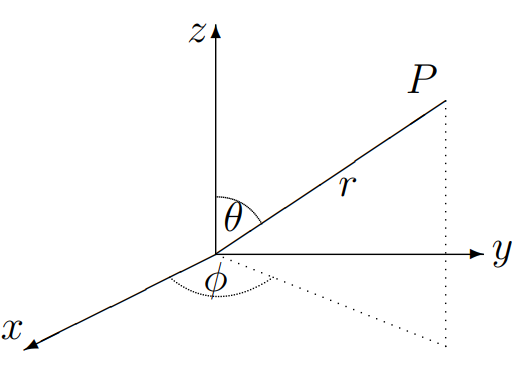
\includegraphics[scale=0.3]{f0.png}
\end{center}

\subsubsection*{Gradient}
The gradient of a \underline{scalar} field
$f(\vc{r})$ is:
$$\dd f(\vc{r})\deq\vc{\nabla}f(\vc{r})\cdot\dd\vc{r}$$
when $\vc{r}\rightarrow\vc{r}+\dd\vc{r}
\implies f\rightarrow f+\dd f$.
Taking the total differential of $f$ yields:
$$\vc{\nabla}f=\sum_{i=1}^{3}\frac{1}{h_i}
\frac{\partial f}{\partial u_i}\vc{e}_i$$
where $\{\vc{e}_i\}$ is \underline{orthogonal}.

\subsubsection*{Divergence}
The divergence of a \underline{vector} field $\vc{F}$ is:
$$\vc{\nabla}\cdot\vc{F}\deq\lim_{\delta V\rightarrow0}
\frac{1}{\delta V}\int_{\delta S}
\vc{F}\cdot\dd\vc{S}$$
for surface $\delta S$ bounds infinitesimal $\delta V$. \\
In orthogonal curvilinear coordinates:
\begin{align*}
    \vc{\nabla}\cdot\vc{F}
    &=\frac{1}{h_1 h_2 h_3}\biggl\{
    \frac{\partial}{\partial u_1}(F_1 h_2 h_3)\;+ \\
    &\frac{\partial}{\partial u_2}(h_1 F_2 h_3)
    +\frac{\partial}{\partial u_3}(h_1 h_2 F_3)
    \biggr\}.
\end{align*}

\subsubsection*{Curl}
The curl of a \underline{vector} field $\vc{F}$
in the \\ direction of unit vector $\hat{\vc{n}}$ is:
$$\hat{\vc{n}}\cdot(\vc{\nabla}\times\vc{F})
\deq\lim_{\delta S\rightarrow0}\frac{1}{\delta S}
\oint_{\delta C}\vc{F}\cdot\dd\vc{r}$$
where curve $\delta C$ encloses plane $\delta S$. \\
In orthogonal curvilinear coordinates:
$$\vc{\nabla}\times\vc{F}
=\frac{1}{h_1 h_2 h_3}
\begin{vmatrix}
    h_1\vc{e}_1 & h_2\vc{e}_2 & h_3\vc{e}_3 \\
    \frac{\partial}{\partial u_1} &
    \frac{\partial}{\partial u_2} &
    \frac{\partial}{\partial u_3} \\
    h_1 a_1 & h_2 a_2 & h_3 a_3
\end{vmatrix}.$$

\subsubsection*{Laplacian}
The Laplacian of a \underline{scalar} field $f$ is:
$$\vc{\nabla}^2 f=\vc{\nabla}\cdot(\vc{\nabla}f)$$
and in orthogonal curvilinear coordinates:
\begin{align*}
    &\vc{\nabla}^2 f
    =\frac{1}{h_1 h_2 h_3}\biggl\{
    \frac{\partial}{\partial u_1}
    \left(\frac{h_2 h_3}{h_1}\frac{\partial f}{\partial u_1}\right)
    + \\
    &\frac{\partial}{\partial u_2}
    \left(\frac{h_3 h_1}{h_2}\frac{\partial f}{\partial u_2}\right)
    +\frac{\partial}{\partial u_3}
    \left(\frac{h_1 h_2}{h_3}\frac{\partial f}{\partial u_3}\right)
    \biggr\}.
\end{align*}
The Laplacian of a \underline{vector} field $\vc{F}$ is:
$$\vc{\nabla}^2\vc{F}=\vc{\nabla}(\vc{\nabla}\cdot\vc{F})
-\vc{\nabla}\times(\vc{\nabla}\times\vc{F}).$$

\subsubsection*{Vector calculus identities}
Particularly for Cartesian coordinates
we can apply the suffix notation:
$$\vc{\nabla}f=
\frac{\partial f}{\partial x_i}\vc{e}_i$$
$$(\vc{u}\cdot\vc{\nabla})\vc{F}
=u_j\frac{\partial}{\partial x_j}F_i$$
$$\vc{\nabla}\cdot\vc{F}=
\frac{\partial F_i}{\partial x_i}$$
$$\vc{\nabla}\times\vc{F}
=\epsilon_{ijk}\frac{\partial F_k}{\partial x_j}
\vc{e}_i$$
$$\frac{\partial x_i}{\partial x_j}=\delta_{ij}
\hspace{0.05in}\text{and}\hspace{0.05in}
\frac{\partial x_i}{\partial x_i}=\delta_{ii}=3.$$
If $\psi$ is a scalar field and $\vc{v}$ a vector field:
$$\vc{\nabla}\times(\vc{\nabla}\psi)=\vc{0}$$
$$\vc{\nabla}\cdot(\vc{\nabla}\times\vc{v})=\vc{0}$$
$$\vc{\nabla}\cdot(\psi\vc{v})
=\vc{\nabla}\psi\cdot\vc{v}+\psi\vc{\nabla}\cdot\vc{v}$$
$$\vc{\nabla}\times(\psi\vc{v})
=\vc{\nabla}\psi\times\vc{v}+\psi\vc{\nabla}\times\vc{v}.$$
Let $\vc{r}=x_i\vc{e}_i$ and $r=(x_i^2)^{1/2}$. Then:
\begin{itemize}
    \item $\displaystyle\vc{\nabla}r=\frac{\vc{r}}{r}
    \hspace{0.05in}\text{and}\hspace{0.05in}
    \vc{\nabla}\left(\frac{1}{r}\right)
    =-\frac{\vc{r}}{r^3}$
    
    \item $\displaystyle\vc{\nabla}r^n
    =n r^{n-2}\vc{r}$
    
    \item $\displaystyle\vc{\nabla}\cdot\vc{r}=3
    \hspace{0.05in}\text{and}\hspace{0.05in}
    \vc{\nabla}\times\vc{r}=\vc{0}$

    \item $\displaystyle\vc{\nabla}\times
    (\vc{c}\times\vc{r})=2\vc{c}$
    
    \item $\displaystyle\vc{\nabla}
    \cdot(\vc{c}\times\vc{r})=\vc{0}$
    for constant $\vc{c}$.
\end{itemize}

\subsubsection*{Divergence theorem}
Let surface $S$ enclose volume $V$. Then:
$$\iiint_V \vc{\nabla}\cdot\vc{F}\dd V
=\oint_S \vc{F}\cdot\dd\vc{S}$$
where $\vc{F}$ is a vector field.

\subsubsection*{Stokes' theorem}
Let closed curve $C$ bound \underline{open} surface $S$
and let $\vc{F}$ be a vector field. Then:
$$\oint_C \vc{F}\cdot\dd\vc{r}
=\iint_S (\vc{\nabla}\times\vc{F})\cdot\dd\vc{S}$$
for $C$ is traversed in anticlockwise sense.

\subsubsection*{Dirac delta function}
The Dirac delta in $1$D is defined as:
$$\delta(x-a)\deq\left\{\begin{array}{ll}
    \infty & x=a \\
    0 & \text{otherwise}.
\end{array}\right.$$
In three dimensions this becomes:
\begin{align*}
    \delta^{(3)}&(\vc{r}-\vc{r}_0)
    \deq\delta(\vc{r}-\vc{r}_0) \\
    &=\delta(x-x_0)\delta(y-y_0)\delta(z-z_0)
\end{align*}
where $(x,y,z)$ are Cartesian coordinates.

In orthogonal curvilinear coordinates:
\begin{align*}
    \delta(\vc{r}-\vc{a})
    =&\frac{1}{h_1 h_2 h_3}\delta(u_1-a_1) \\
    &\cdot\delta(u_2-a_2)\delta(u_3-a_3).
\end{align*}
Importantly we have the \textbf{sift} property:
$$\int_{-\infty}^{\infty}f(x)\delta(x-a)\dd x=f(a)$$
which yields:
$$x\delta(x)=0
\hspace{0.05in}\text{and}\hspace{0.05in}
\delta(cx)=\frac{1}{|c|}\delta(x).$$
If simple solutions of $g(x)=0$ are $x_i$:
$$\int_{-\infty}^{\infty}f(x)\delta(g(x))\dd x
=\sum_i\frac{f(x_i)}{|g'(x_i)|}.$$

\subsubsection*{Coulomb's law}
Consider charges $q$ and $q_1$ at positions
$\vc{r}$ and $\vc{r}_1$.
The force \underline{on} charge $q$ at $\vc{r}$
due to charge $q_1$ at $\vc{r}_1$ is:
$$\vc{F}_1(\vc{r})=\frac{1}{4\pi\epsilon_0}
\frac{q q_1(\vc{r}-\vc{r}_1)}{|\vc{r}-\vc{r}_1|^3}$$
where $q q_1>0$ denotes repulsion.

The permittivity of free space is given by:
$$\epsilon_0=8.85419\times10^{-12}
\text{C}^2\text{N}^{-1}\text{m}^{-2}.$$
Charge has units Coulombs (C) and an electron
has charge $-1.60218\times 10^{-19}$C.

\subsubsection*{Electric fields}
The electric field is induced by a charge distribution
and defined in terms of the
force on a small positive test charge $q$:
$$\vc{E}(\vc{r})\deq\lim_{q\rightarrow0}
\frac{1}{q}\vc{F}.$$
Then for our two charges $q$ and $q_1$:
$$\vc{F}_1(\vc{r})=q\vc{E}_1(\vc{r})$$
where $q_1$ produces electric field $\vc{E}_1$.
$$\therefore\vc{E}_1(\vc{r})
=\frac{1}{4\pi\epsilon_0}
\frac{q_1(\vc{r}-\vc{r}_1)}{|\vc{r}-\vc{r}_1|^3}$$

\subsubsection*{Principle of superposition}
For a set of charges $q_i$ at position $\vc{r}_i$
the total electric field at $\vc{r}$ is:
$$\vc{E}(\vc{r})=\frac{1}{4\pi\epsilon_0}
\sum_i\frac{q_i(\vc{r}-\vc{r}_i)}{|\vc{r}-\vc{r}_i|^3}.$$
For object with \textbf{charge density}
$\rho(\vc{r}')$ its overall electric field at $\vc{r}$ is:
$$\vc{E}(\vc{r})=\frac{1}{4\pi\epsilon_0}
\int_V\rho(\vc{r}')
\frac{\vc{r}-\vc{r}'}{|\vc{r}-\vc{r}'|^3}\dd V'$$
where $\rho(\vc{r}')$ is charge divided by volume.

\subsubsection*{Electrostatic Maxwell's equations}
Because $\displaystyle\vc{\nabla}\left(
\frac{1}{|\vc{r}-\vc{r}'|}\right)
=-\frac{\vc{r}-\vc{r}'}{|\vc{r}-\vc{r}'|^3}$:
$$\vc{E}(\vc{r})=-\vc{\nabla}
\left(\frac{1}{4\pi\epsilon_0}
\int_V\frac{\rho(\vc{r}')}{|\vc{r}-\vc{r}'|}\dd V'\right)$$
and therefore for all \underline{static} electric fields:
$$\vc{\nabla}\times\vc{E}=\vc{0}.$$
$\vc{E}$ is a \textbf{conservative} vector field
where its line integral is \textcolor{red}{in}dependent of path.
Furthermore it may be written as:
$$\vc{E}(\vc{r})=-\vc{\nabla}\phi(\vc{r})$$
for $\phi(\vc{r})$ is the potential of $\vc{E}$.
$$\therefore\phi(\vc{r})=\frac{1}{4\pi\epsilon_0}
\int_V\frac{\rho(\vc{r}')}{|\vc{r}-\vc{r}'|}\dd V'$$
\begin{center}
    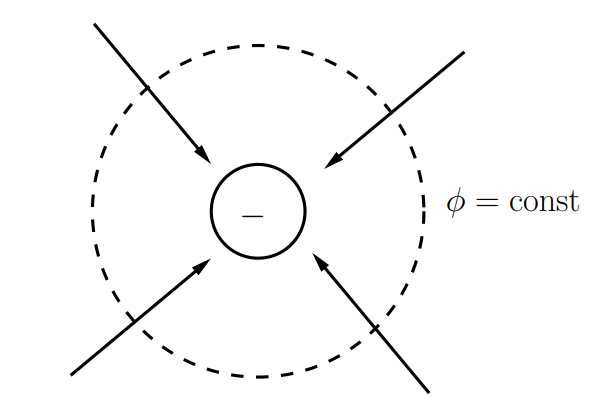
\includegraphics[scale=0.3]{f1.png}
\end{center}
The \textbf{potential difference} between
two points $A$ and $B$ is the energy per unit charge
needed to move a small charge $q$ from $A$ to $B$:
\begin{align*}
    V_{A\rightarrow B}
    &=\lim_{q\rightarrow0}\frac{1}{q}W_{A\rightarrow B} \\
    &=-\frac{1}{q}\int_C\vc{F}\cdot\dd\vc{r} \\
    &=\phi_B-\phi_A.
\end{align*}
A charge distribution $\rho(\vc{r}')$ in an \underline{external}
electric field has potential energy:
$$W=\int_V\rho(\vc{r}')\phi_{ext}(\vc{r}')\dd V'.$$
Because $\displaystyle\vc{\nabla}^2\left(
\frac{1}{|\vc{r}-\vc{r}'|}\right)=-4\pi\delta(\vc{\vc{r}-\vc{r}'})$:
$$\vc{\nabla}\cdot\vc{E}=\frac{\rho(\vc{r})}{\epsilon_0}.$$

\subsubsection*{Electric dipoles}
An electric dipole at $\vc{r}_0$ is defined as two charges
$-q$ at $\vc{r}_0$ and $+q$ at $\vc{r}_0+\vc{d}$
which generates \textbf{dipole moment}:
$$\vc{p}=q\vc{d}$$
and in the \underline{dipole limit} this is defined as:
$$\vc{p}\deq\lim\limits_{\substack{
    q \to \infty \\
    \vc{d} \to \vc{0}}} q\vc{d}$$
known as an ideal dipole.
\begin{center}
    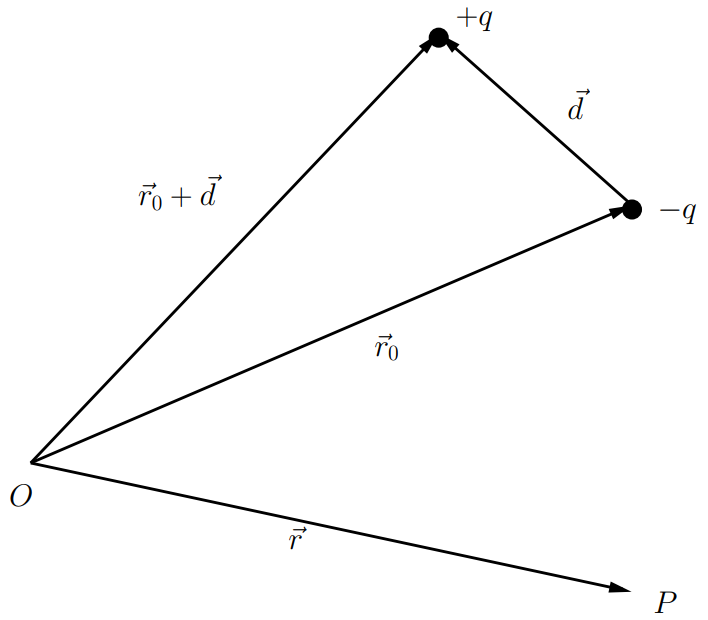
\includegraphics[scale=0.22]{f2.png}
\end{center}

The electrostatic potential
generated by this ideal dipole at $\vc{r}_0$ is given by:
\begin{align*}
    \phi(\vc{r})
    &=\phi_{q}+\phi_{-q} \\
    &=\frac{q}{4\pi\epsilon_0}\left(
    \frac{1}{|\vc{r}-\vc{r}_0-\vc{d}|}
    -\frac{1}{|\vc{r}-\vc{r}_0|}\right) \\
    &\approx\frac{1}{4\pi\epsilon_0}
    \frac{\vc{p}\cdot(\vc{r}-\vc{r}_0)}{|\vc{r}-\vc{r}_0|^3}
\end{align*}
for the first term is expanded in powers of $-\vc{d}$
about $\vc{r}-\vc{r}_0$. 

The electric field generated is:
\begin{align*}
    \vc{E}(\vc{r})
    =&\frac{1}{4\pi\epsilon_0}\bigg[
    -\frac{\vc{p}}{|\vc{r}-\vc{r}_0|^3} \\
    &+\frac{3\vc{p}\cdot(\vc{r}-\vc{r}_0)}{|\vc{r}-\vc{r}_0|^5}
    (\vc{r}-\vc{r}_0)\bigg].
\end{align*}
If the ideal dipole is at the origin:
$$\phi(\vc{r})=\frac{1}{4\pi\epsilon_0}
\frac{\vc{p}\cdot\vc{r}}{r^3}$$
$$\vc{E}(\vc{r})=\frac{1}{4\pi\epsilon_0}
\left(\frac{3\vc{p}\cdot\vc{r}}{r^5}\vc{r}
-\frac{\vc{p}}{r^3}\right).$$
Let ideal dipole moment $\vc{p}$ be parallel to the $z$-axis.
Then in spherical coordinates $(r,\theta,\chi)$,
$\vc{r}=r\vc{e}_r$, $\vc{p}=p\vc{e}_z$ and:
$$\phi(\vc{r})=\frac{p}{4\pi\epsilon_0}\frac{\cos\theta}{r^2}$$
$$\vc{E}(\vc{r})=\frac{p}{4\pi\epsilon_0}\left(
\frac{2\cos\theta}{r^3}\vc{e}_r+\frac{\sin\theta}{r^3}
\vc{e}_{\theta}\right).$$
\begin{center}
    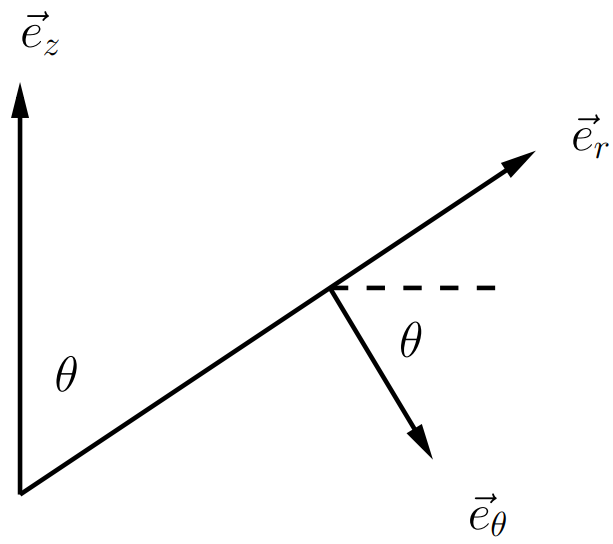
\includegraphics[scale=0.22]{f3.png}
\end{center}

\newcolumn

\subsubsection*{Force, torque and energy}
The \textbf{force} \underline{on} a
\textcolor{red}{dipole at $\vc{r}$}
from external electric field $\vc{E}_{ext}(\vc{r})$ is:
\begin{align*}
    \vc{F}
    &=-q\vc{E}_{ext}(\vc{r})+q\vc{E}_{ext}(\vc{r}+\vc{d}) \\
    &\approx(\vc{p}\cdot\vc{\nabla})\vc{E}_{ext}(\vc{r}).
\end{align*}
The \textbf{torque} \underline{on} a dipole at $\vc{r}$
about the axis $\vc{r}$ due to $\vc{E}_{ext}(\vc{r})$ is:
\begin{align*}
    \vc{G}
    &=\vc{\tau}_{-q}+\vc{\tau}_{q} \\
    &=-q\vc{0}\times\vc{E}_{ext}(\vc{r})
    +q\vc{d}\times\vc{E}_{ext}(\vc{r}+\vc{d}) \\
    &\approx\vc{p}\times\vc{E}_{ext}(\vc{r}).
\end{align*}
The \textbf{energy} of a dipole at $\vc{r}$
from external electric field 
$\vc{E}_{ext}(\vc{r})=-\vc{\nabla}\phi_{ext}(\vc{r})$ is:
\begin{align*}
    W
    &=-q\phi_{ext}(\vc{r})+q\phi_{ext}(\vc{r}+\vc{d}) \\
    &\approx -\vc{p}\cdot\vc{E}_{ext}(\vc{r})
\end{align*}
and $\vc{F}=-\vc{\nabla}W$.

\subsubsection*{Multipole expansion}
Consider object with volume $V$ and charge distribution
$\rho(\vc{r}')$. Let origin be in the object.
Then the potential at $\vc{r}$ is:
\begin{align*}
    \phi(\vc{r})
    &=\frac{1}{4\pi\epsilon_0}\int_V
    \frac{\rho(\vc{r}')}{|\vc{r}-\vc{r}'|}\dd V' \\
    &\approx\frac{1}{4\pi\epsilon_0}\left(
    \frac{Q}{r}+\frac{\vc{p}\cdot\vc{r}}{r^3}
    +\frac{Q_{ij}x_i x_j}{2r^5}\right)
\end{align*}
where $Q$ is the \textbf{total charge} in $V$:
$$Q=\int_V\rho(\vc{r}')\dd V'$$
$\vc{p}$ the \textbf{dipole moment} about the origin:
$$\vc{p}=\int_V\vc{r}'\rho(\vc{r}')\dd V'$$
and $Q_{ij}$ the \textbf{quadrupole tensor}:
$$Q_{ij}=\int_V\rho(\vc{r}')
\bigg[3x'_i x'_j-(r')^2\delta_{ij}\bigg]\dd V'.$$
If $Q\neq0$ then in the far zone ($r\gg r_0$)
the first term (monopole term) dominates.

If $Q=0$ and $\vc{p}=\vc{0}$ then
the third term (quadruple term)
dominates in the far zone and etc.

\subsubsection*{Interaction energy}
By expanding $\phi_{ext}(\vc{r})$ about $\vc{r}=\vc{0}$:
\begin{align*}
    W
    &=\int_V\rho(\vc{r}')\phi_{ext}(\vc{r}')\dd V' \\
    &=Q\phi_{ext}(\vc{0})-\vc{p}\cdot\vc{E}_{ext}(\vc{0}) \\
    &\quad-\frac{1}{6}Q_{ij}\frac{\partial
    \big(\vc{E}_{ext}(\vc{0})\big)_i}
    {\partial x_j}+\dots
\end{align*}
and is the potential energy of a charge \\
distribution $\rho(\vc{r})$ in $\vc{E}_{ext}$.

\newcolumn

\subsubsection*{Gauss' law}
For object with charge distribution
$\rho(\vc{r}')$ and volume $V$ enclosed by surface $S$:
$$\int_S\vc{E}\cdot\dd\vc{S}=\frac{Q_{enc}}{\epsilon_0}$$
where $Q_{enc}$ is total charge enclosed by $V$:
$$Q_{enc}=\int_V\rho(\vc{r}')\dd V'$$
and is useful for symmetric problems.

\subsubsection*{Boundaries}
Let $\sigma$ be the charge density of a surface
separating electric fields $\vc{E}_1$ and $\vc{E}_2$.
\begin{enumerate}
    \item Normal component of electric field is
    \underline{discontinuous} across surface by:
    $$\hat{\vc{n}}\cdot(\vc{E}_2-\vc{E}_1)
    =\frac{\sigma}{\epsilon_0}.$$

    \item Tangential component of electric
    field is continuous across surface:
    $$\vc{E}_{\parallel}\deq\hat{\vc{n}}\times\vc{E}_1
    =\hat{\vc{n}}\times\vc{E}_2.$$
\end{enumerate}

\subsubsection*{Conductors}
Conductors have surplus electrons that can move freely
when an electric field is applied. 
\textbf{In electrostatics}:
\begin{enumerate}
    \item Conductors are in equilibrium,
    all charges are at rest and reside on the
    \underline{surface} of the conductor.

    Hence inside a conductor
    $\rho(\vc{r})=0$, $\vc{E}(\vc{r})=\vc{0}$
    and $\phi=\text{constant}$.

    \item An electric field is always \underline{normal}
    to the surface of a conductor:
    $$E_{\perp}=\frac{\sigma}{\epsilon_0}
    \hspace{0.05in}\text{and}\hspace{0.05in}
    E_{\parallel}=0.$$
\end{enumerate}
The presence of an external electric field induces
a charge distribution $\sigma$ on the surface of our conductor.
This changes the external electric field as it needs to be normal to the surface of the conductor.

\subsubsection*{Poisson's equation}
Because $\vc{E}=-\vc{\nabla}\phi$ and
$\vc{\nabla}\cdot\vc{E}=\rho(\vc{r})/\epsilon_0$:
$$\vc{\nabla}^2\phi=-\frac{\rho(\vc{r})}{\epsilon_0}.$$
We can solve this by direct integration
or using the \textbf{method of images}.

Given volume under consideration place fictitious
charge \underline{outside} the volume such that the system
still satisfies Poisson's equation with boundary conditions.

This potential is our solution.

\newcolumn

\subsubsection*{Electrostatic energy}
The work needed to move point charge $q$
from $\vc{r}_A$ to $\vc{r}_B$ in $\vc{E}(\vc{r})$ is:
$$W_{A\rightarrow B}=q V_{A\rightarrow B}.$$
Then $W_{\infty\rightarrow B}=q\phi(\vc{r}_B)$
since potential $\phi$ vanishes at infinity.

Generalising, the work needed to move a system of
$n$ charges $q_i$ from infinity to $\vc{r}$
is a double sum with overcounting as each charge 
contributes to the electric field:
$$W_e=\frac{1}{2}\frac{1}{4\pi\epsilon_0}
\sum_{i,j (i\neq j)}^{n}\frac{q_i q_j}
{|\vc{r}_j-\vc{r}_i|}.$$

Furthermore the energy needed to move a continuous
charge distribution $\rho(\vc{r}')$ from infinity 
to position $\vc{r}$ is:
\begin{align*}
    W_e
    &=\frac{1}{2}\int_V
    \rho(\vc{r})\phi(\vc{r})\dd V \\
    &=\frac{\epsilon_0}{2}\int_V|\vc{E}(\vc{r})|^2\dd V.
\end{align*}

\subsubsection*{Capacitors}
A capacitor is formed by two conductors 
$1$ and $2$ with equal and opposite charges $Q$ and $-Q$.
The \textbf{capacitance} ($1$CV$^{-1}$) of a
capacitor is defined as:
$$C\deq\frac{Q}{V}$$
where $Q=\sigma A$ for $A$ is the surface area of 
\textcolor{red}{one} conductor and potential
difference $V=\phi_1-\phi_2$ is from polarised conductors.

The energy stored in a capacitor is the amount
of work done to move charge across the two conductors.
So to move charge $\dd q$ from conductor with $+q$:
$$\dd W=\left(\frac{q}{C}\right)\dd q$$
and integrating this up to $Q$ gives:
$$W=\frac{1}{2}\frac{Q^2}{C}.$$

\subsubsection*{Currents}
An elementary current is generated by a charge $q$
moving at velocity $\vc{v}$.

The \textbf{bulk current density} is:
$$\vc{J}(\vc{r})\deq\rho(\vc{r})\vc{v}$$
for $\rho(\vc{r})$ is the volume charge density.

The \textbf{surface current density} is:
$$\vc{K}(\vc{r})\deq\sigma(\vc{r})\vc{v}$$
for $\sigma(\vc{r})$ is the surface charge density.

The \textbf{line charge density} is:
$$\vc{I}(\vc{r})\deq\lambda(\vc{r})\vc{v}$$
for $\lambda(\vc{r})$ is the line charge density.

%\newcolumn

\subsubsection*{Lozentz force}

\subsubsection*{Biot-Savart law}

\subsubsection*{Magnetostatic Maxwell's equations}

\subsubsection*{Amp\`ere's law}
normal and tangent components of conducting surfaces

\subsubsection*{Magnetic dipoles}

\end{multicols*}

\end{document}